\documentclass[a4paper]{article}

\usepackage[utf8]{inputenc}
\usepackage[danish]{babel}
\usepackage [T1]{fontenc}
\usepackage[margin=2.5cm]{geometry}
\usepackage{graphicx}
\usepackage{hyperref}
\usepackage{listings}
\lstset{basicstyle=\footnotesize\ttfamily,breaklines=true}

\title{Introduktion til terminalen\\ for Windows, MacOS X, og Linux\\Udkast!}
\author{Hans Jacob T. Stephensen og Jon Sporring }

\begin{document}
\maketitle

\section{Terminalen}

Som borger i det digitale samfund vi i dag vant til den pæne brugerflade som nutidens populære styresystemer forsyner os med. Som datalog vil man ofte få brug for at tilgå nogle af computerens funktionaliteter som besværliggøres af netop denne brugerflade. Terminalen, som også kaldes kommandolinjen i Windows, er datalogen højre hånd. Terminalen er et simpelt program, som har til formål at tilvejebringe brugeren ønsker i form af tekst-kommandoer. Næsten alle de opgaver, der kan laves med den grafiske brugerflade kan laves i terminalen og omvendt. Vi vil først og fremmest drage nytte af den terminalens direkte kontrol over de programmer, vi skriver, og videre i din uddannelse vil du have gavn af den hurtige og rå information, som man får igennem terminalen.

\section{Den hierarkiske mappestruktur}

Når du åbner en mappe i dit foretrukne styresystem vil mappen have en placering i det aktive filsystem, hvad enten det er fra terminalen eller via operativsystemets grafiske brugergrænseflade. Terminalen vil stort set altid være tilknyttet en bestemt mappe i filsystemet, og man siger at det er den mappe som terminalen "`står"' i. Den præcise struktur som filsystemer har, varierer imellem Linux, MaxOS X og Windows, men fælles er den hierarkiske opbygning. Dette er illustreret i Figure~\ref{fig:filhierakier}.
\begin{figure}
  \begin{center}
    % \scalebox{0.23}
    {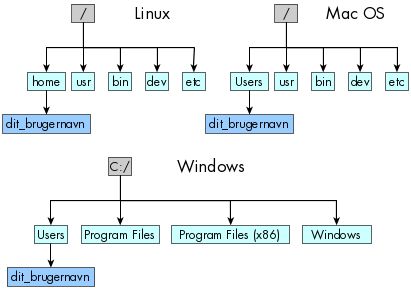
\includegraphics[width=\textwidth]{filehira.png}}
  \end{center}
  \caption{Toppen af filhierarkier i forskellige operativsystemer.}
  \label{fig:filhierakier}
\end{figure}
 Når du begynder at arbejde i terminalen på din nuværende computer er det praktisk både at forestille sig strukturen du kender med mapper og filer i mapper, samt den hierarkiske struktur.

\section{De vigtigste kommandoer}
Der findes et væld af terminalkommandoer, man kan køre fra terminalen, og man kan selv lave yderligere. I det følgende vil vi gennemgå de kommandoer i de 3 forskellige operativsystemet

\subsection{Windows.}
I dette afsnit vil vi gennemgå komandoerne opsummeret i Tabel~\ref{tab:WindowsKommandoer}.
\begin{table}
  \centering
  \begin{tabular}{|l||p{0.5\linewidth}|}
    \hline
    Kommando & Beskrivelse 
    \\ \hline\hline
    \verb|dir|
             & Vis nuværende mappes indhold. 
    \\ \hline
    \verb|cd <mappe>| 
             & få terminalen til at pege på \verb|<mappe>| i stedet for den nuværende mappe. 
    \\ \hline
    % \verb|touch <fil>| & opret en tom fil med navnet \verb|<fil>|. \\ \hline
    %\verb|emacs <fil>|
    %         & Åben \verb|<fil>| i emacs hvis den findes i den nuværende mappe. Findes den ikke oprettes den her automatisk. 
    \\ \hline
    \verb|mkdir <mappe>|
             & opret mappen \verb|<mappe>|. \\ \hline
    \verb|rmdir <mappe>|
             & slet \verb|<mappe>|. \\ \hline
    \verb|move <fil> <nyt filnavn el. mappe>|
             & Flyt \verb|<fil>| ind i \verb|<mappe>|. \\ \hline
    \verb|copy <fil> <nyt filnavn el. mappe>|
             & Opret en ny fil med filnavn \verb|<nyt filnavn>| som en kopi af \verb|<fil>|. \\ \hline
    \verb|del <fil>|
             & slet \verb|<fil>| (Advarsel: Dette kan ikke fortrydes). \\ \hline
    \verb|echo <streng el. variabel>|
               & skriv en streng eller indholdet af en variabel til skærmen. \\ \hline
  \end{tabular}\\
  \caption{Tabel over de vigtigeste kommandoer i Windows kommandoprompt}
  \label{tab:WindowsKommandoer}
\end{table}

Windows 7 og tidligere: Du åbner terminalen ved at trykke på \textit{Start->Run} i nederste venstre hjørne, og derefter skrive \verb|cmd| i boksen. Nu skal der gerne åbnes et terminal vindue med en prompt der viser noget ala
\begin{lstlisting}[frame=single]
Microsoft Windows [Version 6.1.7601]
Copyright (c) 2009 Microsoft Corporation.  All rights reserved.

C:\Users\sporring>
\end{lstlisting}
Hvis du vil se, hvilke filer, som ligger i mappen skriver du
\begin{lstlisting}[frame=single]
C:\Users\sporring>dir
 Volume in drive C has no label.
 Volume Serial Number is 94F0-31BD

 Directory of C:\Users\sporring

30-07-2015  15:23    <DIR>          .
30-07-2015  15:23    <DIR>          ..
30-07-2015  14:27    <DIR>          Contacts
30-07-2015  14:27    <DIR>          Desktop
30-07-2015  17:40    <DIR>          Documents
30-07-2015  15:11    <DIR>          Downloads
30-07-2015  14:28    <DIR>          Favorites
30-07-2015  14:27    <DIR>          Links
30-07-2015  14:27    <DIR>          Music
30-07-2015  14:27    <DIR>          Pictures
30-07-2015  14:27    <DIR>          Saved Games
30-07-2015  17:27    <DIR>          Searches
30-07-2015  14:27    <DIR>          Videos
               0 File(s)              0 bytes
              13 Dir(s)  95.004.622.848 bytes free

C:\Users\sporring>
\end{lstlisting}
hvoraf man kan se, at der er ingen filer og 13 mapper (DIR), dato og tid for deres oprettelse i de 2 venstre kolonner, deres størrelse eller om det er en mappen, samt deres navne i højre kolonne.  De 2 første mapper \verb|.| og \verb|..| findes i hver eneste mappe og henviser til denne mappe samt dens ovenstående. I dette tilfælde er mappen \verb|.| et alias for \verb|C:\Users\sporring| og \verb|..| for \verb|C:\Users|.

Hvis du vil skifte mappe til \verb|Documents| skriver du
\begin{lstlisting}[frame=single]
C:\Users\sporring>cd Documents

C:\Users\sporring\Documents>
\end{lstlisting}
som er den samme mappe, som Windows Explorer finder, når man trykker på \verb|Dokumenter|. På en ny computer er denne mappe typisk tom,
\begin{lstlisting}[frame=single]
C:\Users\sporring\Documents>dir
 Volume in drive C has no label.
 Volume Serial Number is 94F0-31BD

 Directory of C:\Users\sporring\Documents

30-07-2015  19:16    <DIR>          .
30-07-2015  19:16    <DIR>          ..
               0 File(s)              0 bytes
               2 Dir(s)  94.656.716.800 bytes free

C:\Users\sporring\Documents>
\end{lstlisting}
Hvis du vil oprette en ny mappe f.eks.\ med navn \verb|minMappe|, der hvor du står, skriver du
\begin{lstlisting}[frame=single]
C:\Users\sporring\Documents>mkdir minMappe

C:\Users\sporring\Documents>dir
 Volume in drive C has no label.
 Volume Serial Number is 94F0-31BD

 Directory of C:\Users\sporring\Documents

30-07-2015  19:17    <DIR>          .
30-07-2015  19:17    <DIR>          ..
30-07-2015  19:17    <DIR>          minMappe
               0 File(s)              0 bytes
               3 Dir(s)  94.656.638.976 bytes free

C:\Users\sporring\Documents>
\end{lstlisting}
Vi kan oprette en fil \verb|echo| og \textit{redirection},
\begin{lstlisting}[frame=single]
C:\Users\sporring\Documents>echo "Hej" > hej.txt

C:\Users\sporring\Documents>dir
 Volume in drive C has no label.
 Volume Serial Number is 94F0-31BD

 Directory of C:\Users\sporring\Documents

30-07-2015  19:18    <DIR>          .
30-07-2015  19:18    <DIR>          ..
30-07-2015  19:17    <DIR>          minMappe
30-07-2015  19:18                 8 hej.txt
               1 File(s)              8 bytes
               3 Dir(s)  94.656.634.880 bytes free

C:\Users\sporring\Documents>
\end{lstlisting}
Hvis vi nu gerne vil flytte filen \verb|hej.txt| til mappen \verb|minMappe| gør man som følger,
\begin{lstlisting}[frame=single]
C:\Users\sporring\Documents>move hej.txt minMappe
        1 file(s) moved.

C:\Users\sporring\Documents>
\end{lstlisting}
og endeligt, hvis man ønsker at slette filen og derefter mappen skriver man
\begin{lstlisting}[frame=single]
C:\Users\sporring\Documents>cd minMappe

C:\Users\sporring\Documents\minMappe>del hej.txt

C:\Users\sporring\Documents\minMappe>cd ..

C:\Users\sporring\Documents>rmdir minMappe

C:\Users\sporring\Documents>dir
 Volume in drive C has no label.
 Volume Serial Number is 94F0-31BD

 Directory of C:\Users\sporring\Documents

30-07-2015  19:20    <DIR>          .
30-07-2015  19:20    <DIR>          ..
               0 File(s)              0 bytes
               2 Dir(s)  94.651.142.144 bytes free

C:\Users\sporring\Documents>
\end{lstlisting}
De kommandoer, man kan køre fra kommandolinjen, skal være indbygget eller i terminalens søgesti. Man kan se, hvad søgestien er ved at skrive
\begin{lstlisting}[frame=single]
C:\Users\sporring\Documents>echo %Path%
C:\Windows\system32;C:\Windows;C:\Windows\System32\Wbem;C:\Windows\System32\WindowsPowerShell\v1.0\;"\Program Files\emacs-24.5\bin\"

C:\Users\sporring\Documents>
\end{lstlisting}
og stien kan ændres ved at gå ind i Kontrolpanelet og vælge \verb|System and Security| $\rightarrow$ \verb|System| $\rightarrow$ \verb|Advanced system settings| $\rightarrow$ \verb|Environment Variables| og i \verb|System variables| boksen dobbeltklikke på \verb|Path| og tilføje eller fjerne en sti i dens liste. Stiens elementer adskilles af "`;"'. Vær opmærksom på, at Windows afhænger af denne indstilling, så fjerne kun stier, som du er sikker på ikke skal bruges til noget.

En nyttig feature i terminalen er, at den kan gætte på, hvad man er ved at skrive, ved at trykke \verb|tab|, hvorpå resten af kommandoen ofte vil blive automatisk færdiggjort.

\subsection{MacOS X og Linux}
MacOS X (OSX) og Linux har mange lighedpunkter. I dette afsnit vil vi gennemgå de vigtigeste kommandoer i terminalen, \verb|bash|, som er standard terminal i OSX og mange Linux versioner. En opsummering ses i Tabel~\ref{tab:bashKommandoer}.
\begin{table}
  \centering
  \begin{tabular}{|l||p{0.5\linewidth}|}
    \hline
    Kommando & Beskrivelse 
    \\ \hline\hline
    \verb|ls| 
             & Vis nuværende mappes indhold. 
    \\ \hline
    \verb|cd <mappe>| 
             & få terminalen til at pege på \verb|<mappe>| i stedet for den nuværende mappe. 
    \\ \hline
    % \verb|touch <fil>| & opret en tom fil med navnet \verb|<fil>|. \\ \hline
    %\verb|emacs <fil>|
    %         & Åben \verb|<fil>| i emacs hvis den findes i den nuværende mappe. Findes den ikke oprettes den her automatisk. 
    \\ \hline
    \verb|mkdir <mappe>| 
             & opret \verb|<mappe>|. \\ \hline
    \verb|rmdir <mappe>|
             & slet \verb|<mappe>|. \\ \hline
    \verb|mv <fil> <nyt filnavn el. mappe>|
             & Flyt \verb|<fil>| ind i \verb|<mappe>|. \\ \hline
    \verb|cp <fil> <nyt filnavn el. mappe>|
             & Opret en ny fil med filnavn \verb|<nyt filnavn>| som en kopi af \verb|<fil>|. \\ \hline
    \verb|rm <fil>|
             & slet \verb|<fil>| (Advarsel: Dette kan ikke fortrydes). \\ \hline
    \verb|echo <streng el. variabel>|
             & skriv en streng eller indholdet af en variabel til skærmen. \\ \hline
  \end{tabular}\\
  \caption{Tabel over de vigtigeste kommandoer i Bash terminalen}
  \label{tab:bashKommandoer}
\end{table}

I OSX finder du terminalen ved at åbne \verb|Finder| og navigere til \verb|Applications| $\rightarrow$ \verb|Utilities| -> \verb|Terminal|. 

I Linux kan du åbner en terminal ved at taste \verb|Ctrl + Alt + T| (Andre Linux distributioner kan have anden tast kombination. f.eks. \verb|Super + T|). 

Når du har åbnet terminalen blive du vist et vindue, hvori der står noget ala
\begin{lstlisting}[frame=single]
Last login: Thu Jul 30 11:52:07 on ttys000
FN11194:~ sporring$ 
\end{lstlisting}
Hvis du vil se, hvilke filer, som ligger i mappen skriver du
\begin{lstlisting}[frame=single]
FN11194:~ sporring$ ls
Applications	Documents	Library		Music		Public
Desktop		Downloads	Movies		Pictures
FN11194:~ sporring$ 
\end{lstlisting}
"`FN11194"' er navnet på computeren, tegnet $\sim$ bruges i Linux til at angive din egen Home-mappe, og "`sporring"' er brugernavnet for den som er logget på. Man kan få yderligere detaljer ved at skrive
\begin{lstlisting}[frame=single]
FN11194:~ sporring$ ls -la .
drwx------   6 sporring  staff   204 Jul 30 14:07 Applications
drwx------+ 32 sporring  staff  1088 Jul 30 14:34 Desktop
drwx------+ 76 sporring  staff  2584 Jul  2 15:53 Documents
drwx------+  4 sporring  staff   136 Jul 30 14:35 Downloads
drwx------@ 63 sporring  staff  2142 Jul 30 14:07 Library
drwx------+  3 sporring  staff   102 Jun 29 21:48 Movies
drwx------+  4 sporring  staff   136 Jul  4 17:40 Music
drwx------+  3 sporring  staff   102 Jun 29 21:48 Pictures
drwxr-xr-x+  5 sporring  staff   170 Jun 29 21:48 Public
FN11194:~ sporring$ 
\end{lstlisting}
hvorved man ud fra venstre kolonne kan lære at alle navnene er kataloger (d) og at du men ingen andre læse, skrive og adgang til mapperne (rwx). Informationen i den næste kolonne kan oftes ignoreres, men viser hvor mange links der er til denne fil eller mappe, derefter kommer ejeren af filenens brugernavn og brugergruppe, her sporring og staff, så filen eller mappens størrelse, dato og tidsstempel for hvor filen eller mappen senest er blevet ændret, og til sidst fil- eller mappenavnet.  Der er også altid 2 skjulte mapper, \verb|.| og \verb|..|, hvor \verb|.| et alias for \verb|C:\Users\sporring| og \verb|..| for \verb|C:\Users|.

Hvis du vil skifte mappe til \verb|Documents| skriver du
\begin{lstlisting}[frame=single]
FN11194:~ sporring$ cd Documents/
FN11194:Documents sporring$ 
\end{lstlisting}
som er den samme mappe, som man kan finde ved at trykker på \verb|Dokumenter| i det grafiske brugergrænseflade. Bemærk, at nogle systemet oversætter standard filnavne således at deres navne skrives på forskellige sprog i den grafiske brugergrænseflade og i terminalen. På en ny computer er denne mappe typisk tom,
\begin{lstlisting}[frame=single]
FN11194:Documents sporring$ ls
FN11194:Documents sporring$  
\end{lstlisting}
Hvis du vil oprette en ny mappe f.eks.\ med navn \verb|minMappe|, der hvor du står, skriver du
\begin{lstlisting}[frame=single]
FN11194:Documents sporring$  mkdir minMappe
FN11194:Documents sporring$ ls
minMappe
FN11194:tmp sporring$  
\end{lstlisting}
Vi kan oprette en fil \verb|echo| og \textit{redirection},
\begin{lstlisting}[frame=single]
FN11194:Documents sporring$ echo "hej" > hej.txt
FN11194:Documents sporring$ ls
hej.txt		minMappe
\end{lstlisting}
Hvis vi nu gerne vil flytte filen \verb|hej.txt| til mappen \verb|minMappe| gør man som følger,
\begin{lstlisting}[frame=single]
FN11194:Documents sporring$ echo mv hej.txt minMappe/
FN11194:Documents sporring$ 
\end{lstlisting}
og endeligt, hvis man ønsker at slette filen og derefter mappen skriver man
\begin{lstlisting}[frame=single]
FN11194:Documents sporring$ cd minMappe/
FN11194:minMappe sporring$ rm hej.txt 
FN11194:minMappe sporring$ cd ..
FN11194:Documents sporring$ rmdir minMappe/
FN11194:Documents sporring$ ls
FN11194:Documents sporring$ 
\end{lstlisting}
De kommandoer, man kan køre fra kommandolinjen, skal være indbygget eller i terminalens søgesti. Man kan se, hvad søgestien er ved at skrive
\begin{lstlisting}[frame=single]
FN11194:Documents sporring$ echo $PATH
/Applications/Maple 17/:/Applications/PackageMaker.app/Contents/MacOS/:/Applications/MATLAB_R2014b.app/bin/:/opt/local/bin:/opt/local/sbin:/usr/local/bin:/usr/bin:/bin:/usr/sbin:/sbin:/opt/X11/bin:/Library/TeX/texbin
FN11194:Documents sporring$ 
\end{lstlisting}
og stien kan ændres ved at editere opsætningsfilen for bash. På OSX hedder den \verb|~/.profile| mens på Linux kan den hedde enten \verb|~/.bash_profile| eller \verb|~/.bashrc|. I den kan man tilføje nye stier ved at indsætte en linje med \verb|export PATH="<min nye sti>:<min anden nye sti>:$PATH"|.

En nyttig feature ved Bash er, at terminalen til at gætte på, hvad man er ved at skrive, ved at trykke \verb|tab|, hvorpå resten af kommandoen ofte vil blive automatisk færdiggjort. Desuden kan manualer til de fleste kommandoer kan findes ved at skrive \verb|man| foran kommandoen. Manualen til \verb|rm| kan f.eks. fås ved at skrive \verb|man rm|.

% \subsection{Linux.}
% Hvis du i din Home-mappe opretter en mappe \verb|studie| med en undermappe \verb|pop|, igen med undermapper \verb|noter| og \verb|uge1|, samt en fil med navnet \verb|terminalNoter.txt|, så kan din terminal f.eks. se således ud:

% \begin{lstlisting}[frame=single, language=bash]
% bruger@computer:~$ mkdir studie
% bruger@computer:~$ cd studie/
% bruger@computer:~/studie$ mkdir pop
% bruger@computer:~/studie$ cd pop/
% bruger@computer:~/studie/pop$ mkdir uge1
% bruger@computer:~/studie/pop$ mkdir noter
% bruger@computer:~/studie/pop$ ls noter  terminalNoter.txt  uge1
% bruger@computer:~/studie/pop$ mv terminalNoter.txt noter/
% bruger@computer:~/studie/pop$
% \end{lstlisting}
% Ønsker du derpå at skrive i documented \verb|terminalNoter.txt| kan du directe fra din home mappe skrive
% \begin{verbatim}
% bruger@computer:~$ emacs studie/pop/noter/terminalNoter.txt
% \end{verbatim}
% eller alternativt få terminalen til først at pege på mappen \verb|noter| og derpå åbne documentet ved
% \begin{verbatim}
% bruger@computer:~$ cd studie/pop/noter/
% bruger@computer:~/studie/pop/noter$ emacs terminalNoter.txt
% \end{verbatim}

% \section{Compilering af \verb|F\#| programmer}

% \subsection{Linux.}

% Hvis \verb|F\#| er succesfuld installeret på din maskine, kan du i terminalen skrive \verb|fsharpi|.
% Pg har du skrevet et program i en kildekode fil med navnet \verb|mitprogram.fsx| kan du oversætte det til maskinkode ved at i terminalen at skrive \verb|fsharpc mitprogram.fsx| - hvortil en ny eksekverbar fil med navnet \verb|mitprogram.exe| vil blive skrevet til samme mappe. Hvis compileringen er en succes vil din terminal have følgende stående:

% \begin{verbatim}
% bruger@computer:~$ fsharpc mitprogram.fsx
% F# Compiler for F# 3.1 (Open Source Edition)
% Freely distributed under the Apache 2.0 Open Source License
% bruger@computer:~$
% \end{verbatim}

% \subsection{MacOS X.}

% [OBS: MANGLER]

% \subsection{Windows.}

% [OBS: MANGLER]


\end{document}